\documentclass[a4paper,12pt]{article}
\usepackage[utf8x]{inputenc}
\usepackage{amssymb}
\usepackage{amsfonts}
\usepackage{mathrsfs}
\usepackage{amsmath}
\usepackage{amsthm}
\usepackage[margin=2cm]{geometry}
\usepackage{times}
\usepackage{graphicx}
\usepackage{enumitem}
\usepackage{fancyhdr}
\usepackage{hyperref}
\usepackage{setspace}
\usepackage{subcaption}
\usepackage{mathtools}

% stuff added by Cian
\usepackage{lineno}
\linenumbers
\renewcommand{\baselinestretch}{1.5}
\usepackage{authblk}

% biliography stuff
%\usepackage[
%backend=biber,
%style=alphabetic,
%sorting=ynt
%]{biblatex}

%\addbibresource{calcium_imaging_model_refs.bib}

\newtheorem{theorem}{Theorem}
\newtheorem{proposition}{Proposition}[section]
\newtheorem{lemma}{Lemma}[section]
\newtheorem{corollary}{Corollary}[section]
\theoremstyle{definition}
\newtheorem{definition}{Definition}[section]

\newcommand{\boldnabla}{\mbox{\boldmath$\nabla$}} % to be used in mathmode
\newcommand{\cbar}{\overline{\mathbb{C}}}% to be used in mathmode
\newcommand{\diff}[2]{\frac{d #1}{d #2}}% to be used in mathmode
\newcommand{\difff}[2]{\frac{d^2 #1}{d #2^2}}% to be used in mathmode
\newcommand{\pdiff}[2]{\frac{\partial #1}{\partial #2}} % to be used in mathmode
\newcommand{\pdifff}[2]{\frac{\partial^2 #1}{\partial #2^2}}% to be used in mathmode
\newcommand{\upperth}{$^{\mbox{\footnotesize{th}}}$}%to be used in text mode
\newcommand{\vect}[1]{\mathbf{#1}}% to be used in mathmode
\newcommand{\curl}[1]{\boldnabla \times \vect{#1}} % to be used in mathmode
\newcommand{\divr}[1]{\boldnabla \cdot \vect{#1}} %to be used in mathmode
\newcommand{\modu}[1]{\left| #1 \right|} %to be used in mathmode
\newcommand{\brak}[1]{\left( #1 \right)} % to be used in mathmode
\newcommand{\comm}[2]{\left[ #1 , #2 \right]} %to be used in mathmode
\newcommand{\dop}{\vect{d}} %to be used in mathmode
\newcommand{\cov}{\text{cov}} %to be used in mathmode
\newcommand{\var}{\text{var}} %to be used in mathmode
\newcommand{\mb}{\mathbf} %to be used in mathmode
\newcommand{\bs}{\boldsymbol} %to be used in mathmode
% Title Page
\title{Sensitivity of the spikes-to-fluorescence transform to calcium indicator and neuron properties}
\date{}

\author[1]{Thomas J. Delaney}
\author[2]{Michael C. Ashby}
\author[1]{Cian O'Donnell}
\affil[1]{School of Computer Science, Electrical and Electronic Engineering, and Engineering Mathematics, University of Bristol, Bristol, United Kingdom.}
\affil[2]{School of Physiology, Pharmacology and Neuroscience, University of Bristol, Bristol, United Kingdom.}
\renewcommand\Affilfont{\itshape\small}

\begin{document}

\maketitle

\abstract{Fluorescent calcium indicators such as GCaMP are widely used to monitor neuronal activity. However the relationship between the fluorescence signal and the underlying action potential firing is poorly understood. This lack of knowledge makes it difficult for experimenters to decide between different indicator variants for a given application. We addressed this problem by studying a basic biophysical model of calcium dynamics in neuronal soma. We fit the model parameters to publicly available data where GCaMP6s fluorescence and whole-cell electrophysiological recordings were made simultaneously in the same single neurons. We systematically varied the model’s parameters to characterise the sensitivity of spike train inference algorithms to the calcium indicator’s main biophysical properties: binding rate, dissociation rate, and molecular concentration. This model should have two potential uses: experimental researchers may use it to help them select the optimal indicator for their desired experiment; and computational researchers may use it to generate simulated data to aid design of spike inference algorithms.}

\section{Introduction}
Although fluorescent calcium indicators such as GCaMP are widely used to monitor neuronal activity, the relationship between the fluorescence signal and the underlying action potential firing is imperfect. The fluorescence signal has a low signal-to-noise ratio, and most indicators' kinetics are slow relative to the millisecond-timescale dynamics of the membrane voltage (example in Figure 1). This makes spike inference difficult. Furthermore, the effects of the indicator and cell properties on the fluorescence signal are unknown. For example, genetically encoded indicators can accumulate within neurons over weeks and months \cite{chen}. Studies using calcium-sensitive fluorescent dyes have shown that indicator concentration has substantial effects on the spike-to-fluorescence relationship \cite{maravall}. Therefore spike rates inferred from GCaMP fluorescence signals may give misleading results if comparing across imaging sessions. More generally, the poor understanding of the spike-to-fluorescence transform means experimenters may not know whether to trust the outputs of spike train inference methods in any given application.

\begin{figure}[h]
    \centering
    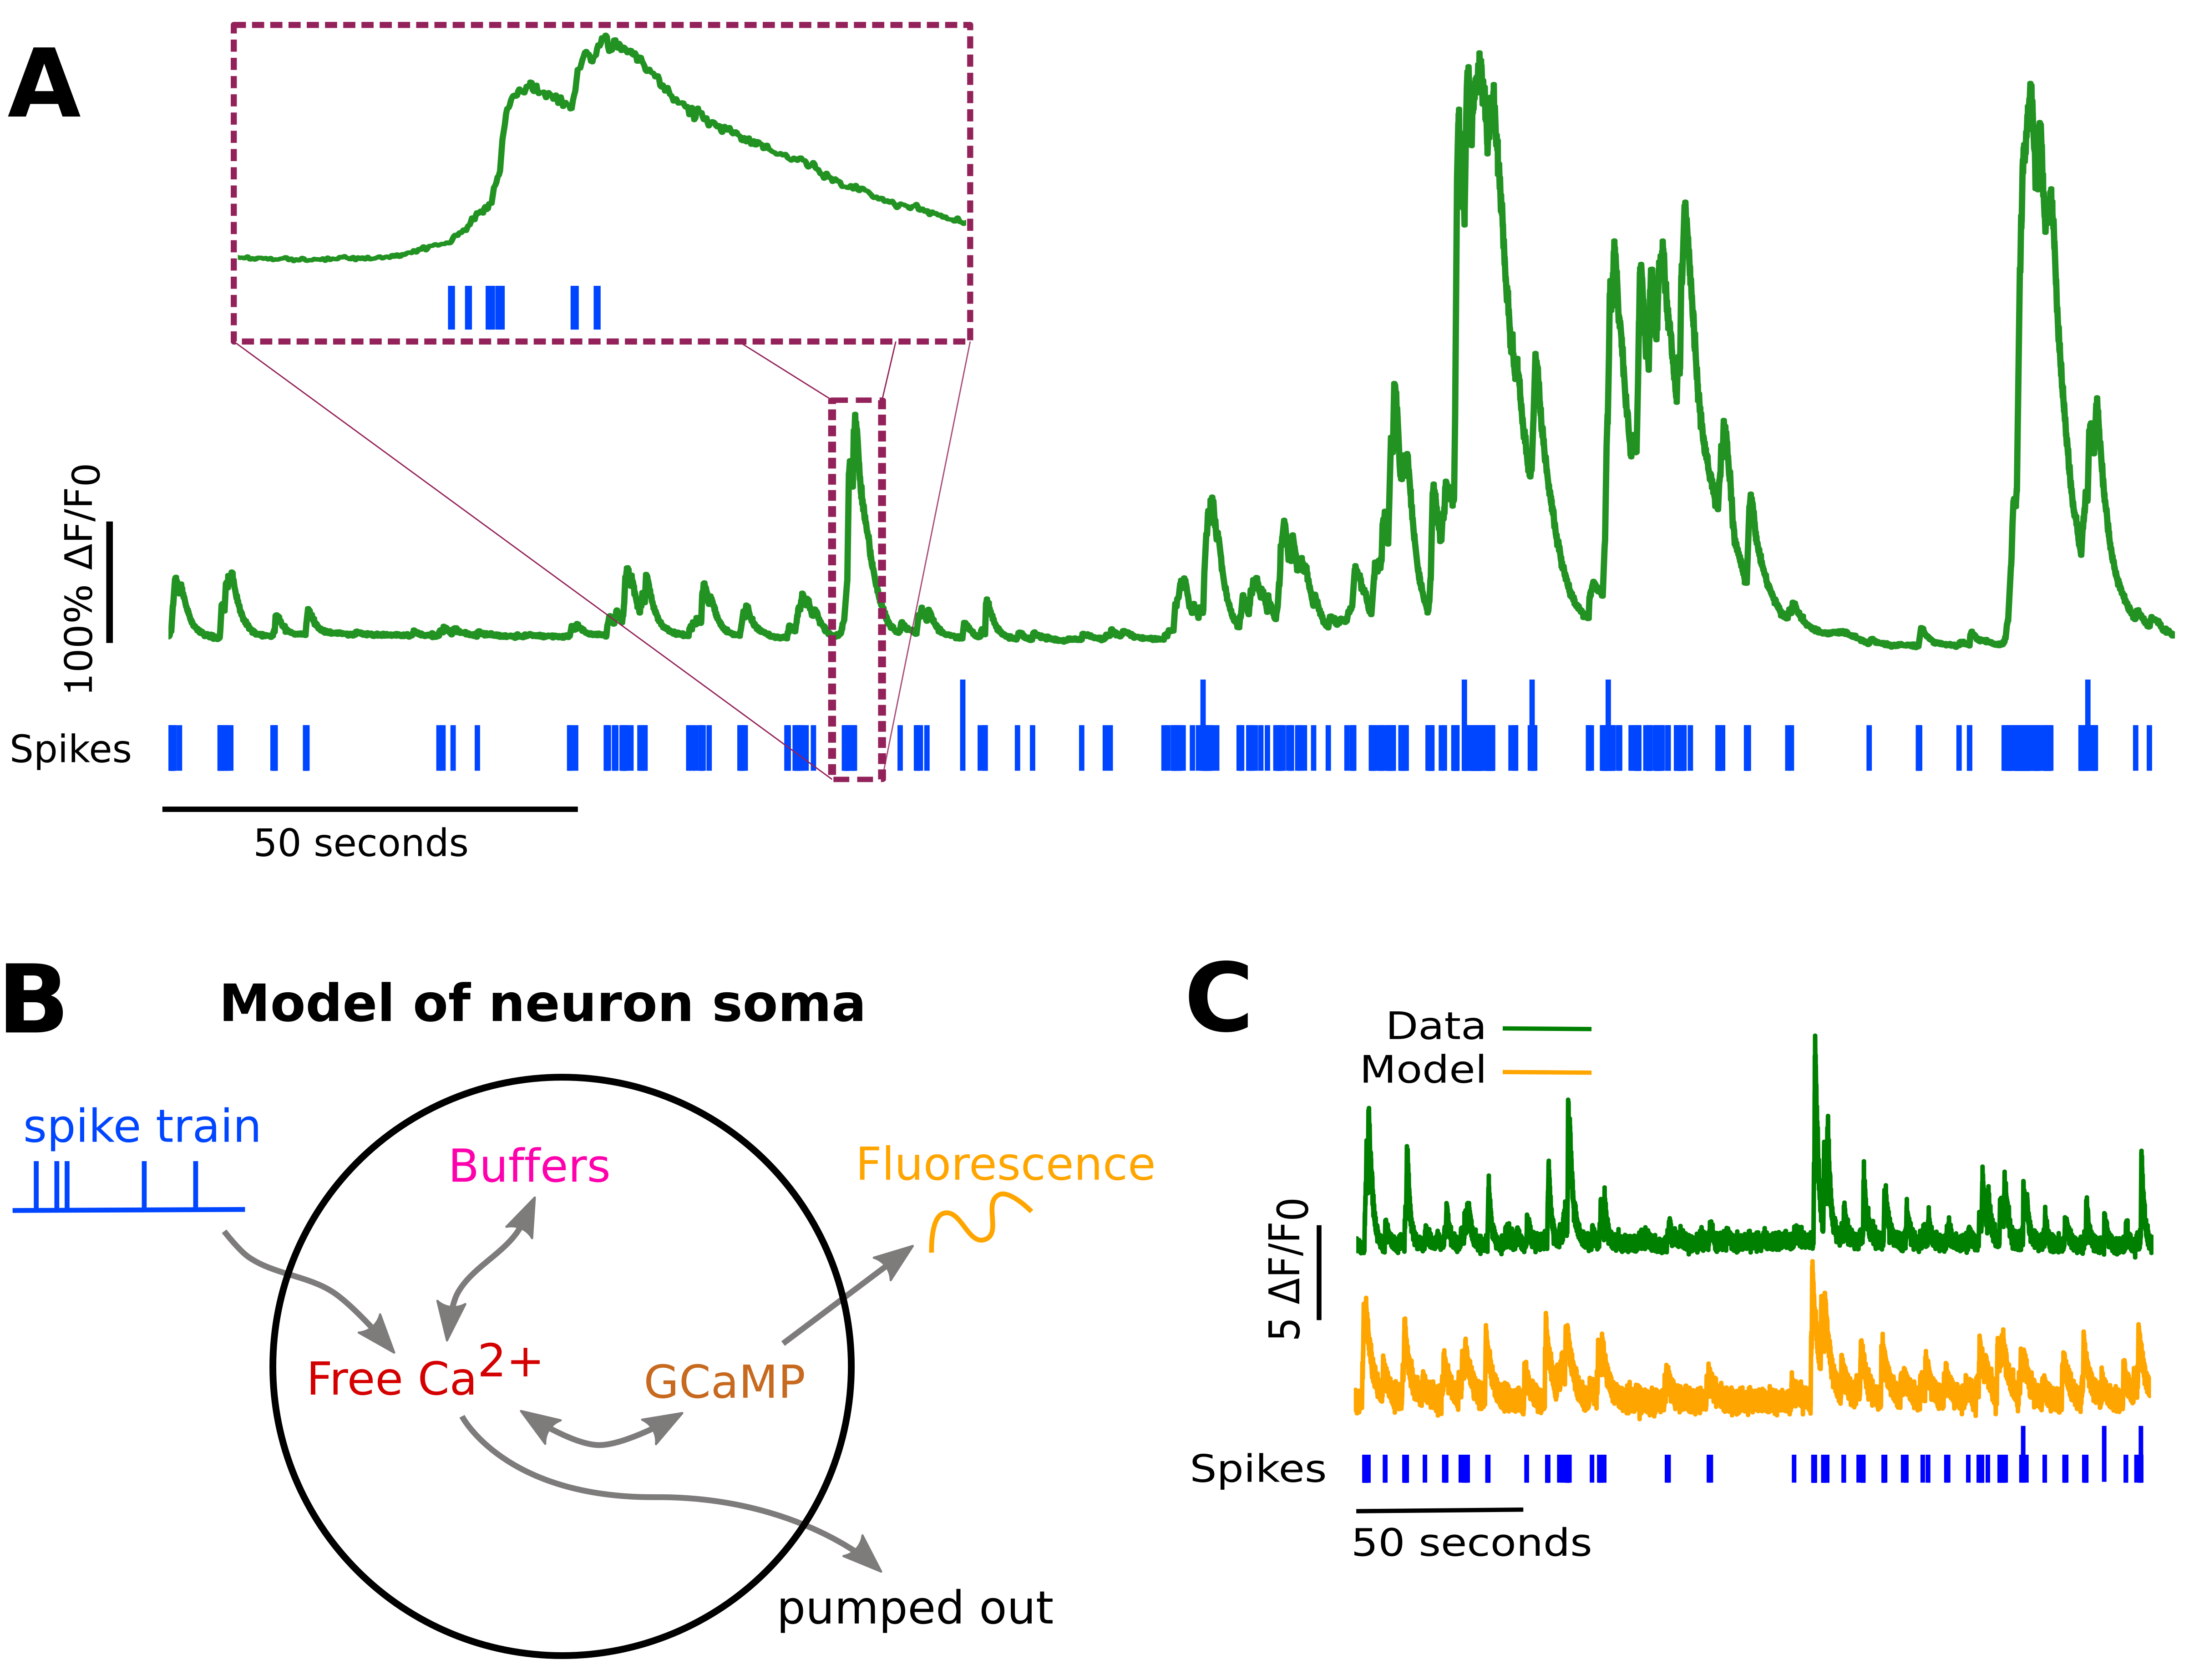
\includegraphics[width=\textwidth]{figures/Figure1.png}
  \caption{\\ A: Example spike train (blue) and the corresponding GCaMP6s fluorescence trace (green), data replotted from \cite{berens}. Inset shows zoomed section of traces to highlight slow decay of GCaMP6s fluorescence relative to spike time intervals.\\
  B: Schematic diagram of the neuron calcium and GCaMP computational model.\\
  C: Good visual match of data fluorescence trace (green) and model simulated fluorescence (orange) in response to an identical spike train (blue).}
  \label{fig:spike_finder_example}
\end{figure}

Spike trains are usually inferred from the time series of intensity values of one pixel of the fluorescence image, where the pixel is located at the cell's soma. The problems of identfying these pixels, and inferring spikes from their time series can solved separately or together. When attempting to infer spikes, the fluorescence trace is modelled as a linear combination of calcium concentration dynamics, a baseline calcium concentration, and some Gaussian noise. The calcium concentration dynamics are modelled as an autoregressive process of degree $1$ or $2$ with a pulse input corresponding to the spike train, or the number of spikes fired in a time step. The model includes no dynamics for the fluorescent indicator itself. Furthermore, in order to make this model into an easily solvable linear programming problem the number of spikes fired in a timestep is not restricted to non-negative integers but to arbitrary non-negative values\cite{vogelstein, pnevmatikakis, friedrich, paninski1, paninski2}. More biologically inspired spike inference models do exist\cite{deneux}, but their fundamentals are very similar. In this work, we investigated the effect of changing dynamics and buffer concentrations on the accuracy of the inference algorithms based on these models.

The aim of this project was to model the fluorescence traces produced by a fluorescent calcium indicator in a neuron soma resulting from a specific spike train, given calcium indicator parameters such as binding rate, dissociation rate, and molecular concentration. Such a model would allow benchmarking of various spike inference algorithms, and enable understanding of how indicator characteristics affect the quality of spike train inference.

The model we developed consisted of free calcium, fluorescent indicator molecules, and mobile and immobile endogenous calcium buffers. The indicator molecules which were bound to a calcium molecule could be either excited, i.e. able to release a photon, or relaxed. In order to reproduce the noise inherent in the data collection, we modelled the release of photons from the excited indicator bound calcium as a stochastic process.

The fluorescence traces produced by the simulation were calibrated to reproduce the signal-to-noise ratio observed in experimental data. Previously published spike inference algorithms were then used to infer spike trains from the experimental fluorescence traces and the modelled fluorescence traces. The parameters of the model were then varied in order to determine the effect on the system dynamics and the effects on spike inference.

\section{Results}
\subsection{A biophysical computational model can generate accurate fluorescence traces from spike trains}
To study the relationship between action potential firing and calcium fluorescence, we built a computational model of calcium dynamics in a neuronal soma. The model consisted of four dynamic variables: the concentration of free calcium, two types of endogenous buffer, and the calcium-sensitive fluorescent indicator. Each of the buffers and the indicator could independently bind and unbind with calcium. These reactions were modelled as
\begin{align*}
   [X][Ca^{2+}] \xrightleftharpoons[k_{Xb}]{k_{Xf}} [XCa]
\end{align*}
where $X$ is the buffer concentration and $Ca^{2+}$ is the calcium concentration. Each species could therefore exist in two states: either bound with calcium or unbound. To model the imaging process, we also added a third, excited state to the indicator. When in the calcium-bound state, the indicator could be converted to an excited state, corresponding to the absorption of a photon. The rate of this excitation process could be interpreted as the intensity of the light illuminating the sample. Once excited, the species decayed back to the unexcited state at a fixed rate, corresponding to the spontaneous emission of photons. The total emitted fluorescence signal was interpreted as proportional to this de-excitation flux. To represent experimental noise in the photon capture process, we drew a random number of captured photons at each time step from a binomial distribution, parameterised by a number $p$ that corresponds to the mean fraction of released photons that are captured.

The model had 17 parameters in total describing the molecules’ concentrations and reaction rates (Methods). We set 13 of these parameters to values from the literature. The remaining 4 parameter values we fit to publicly-available data \cite{berens}, briefly explained as follows (see Methods for full details).  Single neurons from acute rat cortical slices expressing GCaMP6f were imaged with two-photon microscopy while the membrane potentials of the somata of the same neurons were simultaneously recorded via whole-cell patch clamp electrophysiology. In this dataset, the electrical recordings give unambiguous information about neurons' spike times. To do the parameter fitting, we feed these spike trains as inputs to the computational model. After running, the model returns a simulated fluorescence trace. We aimed to find the model parameter values that give the best match between this simulated fluorescence trace and the real fluorescence time series recorded in the corresponding neuron. To do this we used a suite of optimisation procedures to jointly fit both the real neuron’s fluorescence time series and power spectrum, which capture complementary information about the spikes-to-fluorescence mapping (Methods). We performed the fitting procedure independently for each of the $20$ neurons in the spikefinder dataset (http://spikefinder.org). After fitting, the model produced realistic-looking fluorescence time series (Figure \ref{fig:spike_finder_example}).

\subsection{Spike inference algorithms perform similarly on real data compared with time series simulated from the model}
Researchers often pass the fluorescence time series through a spike inference tool before performing further statistical analyses. These spike inference algorithms take the fluorescence trace as input and attempt to estimate the neuronal spike train that triggered them\cite{vogelstein, pnevmatikakis, friedrich, paninski1, paninski2, deneux}. Part of our motivation for building this model was to allow us to ask the question: how do the properties of the cell and the calcium indicator affect the quality of spike inference? In order to trust the conclusions from our model, we should first be confident that spike inference from our simulated fluorescence traces is similar to that from the real data. To test this we passed each of the simulated fluorescence traces through three previously published spike inference algorithms, quantified their performance against the ground-truth electrophysiology data, repeated the procedure for the real calcium fluorescence time series, and compared the accuracy of the inference processes in all cases. The \textit{true positive rate}, also known as the \textit{recall}, the \textit{sensitivity}, or the \textit{probability of detection} of spike inference varied across the three inference algorithms we tried (p value and statistical test here). The constrained non-negative matrix deconvolution algorithm \cite{pnevmatikakis} (CNMD algorithm) correctly detected approximately $45\%$ of the true spikes, the OASIS algorithm \cite{friedrich} correctly detected approximately $35\%$ of the true spikes, and the ML spike algorithm \cite{deneux} correctly detected approximately $15\%$ of the true spikes (see figure \ref{fig:three_algo_comparison}). Notably, for two of the three inference algorithms, the quality of inference was also fairly consistent for individual spike trains, not just the group means ($p > 0.05$, paired t-test). This demonstrates that the models were generating fluorescence time series that were similarly difficult to decode as the real data, in ways that were not specific to any one inference algorithm. This is evidence that the models captured real aspects of the spikes-to-fluorescence transform.
\begin{figure}[h]
\centering
  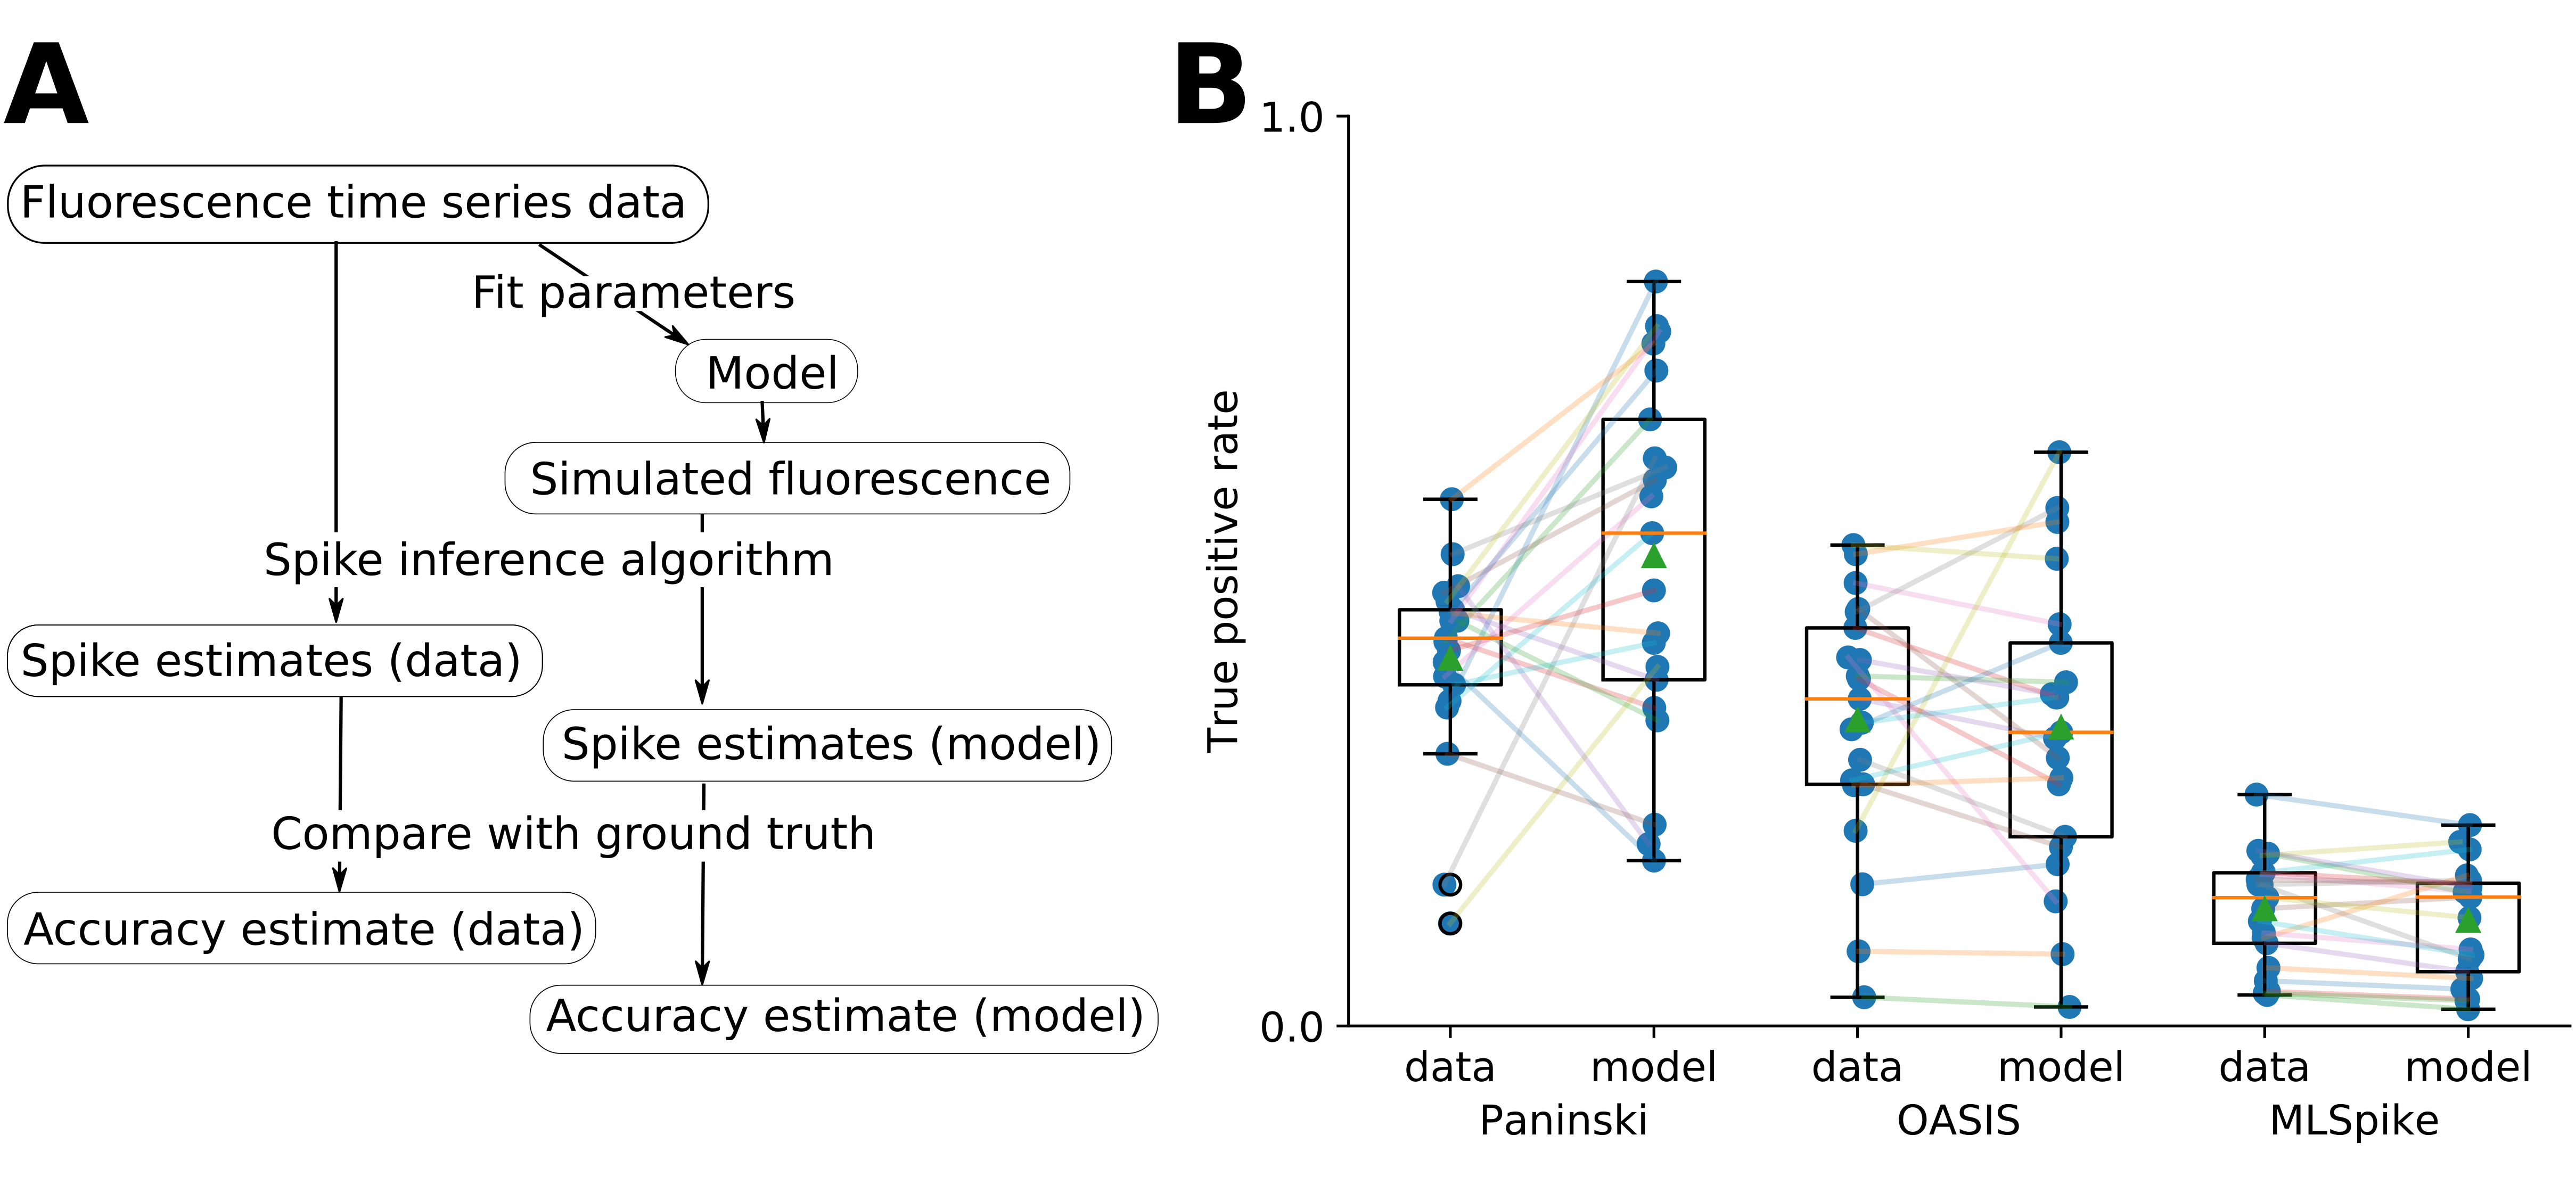
\includegraphics[width=\textwidth]{figures/Figure2.png}
  \caption{\\
  A: Workflow to compare spike inference for real versus simulated fluorescence data.\\
  B: True positive rates achieved by three different spike inference algorithms when applied to observed spike trains, and simulated spike trains. Data points overlaid as blue circles. The performance is similar from real and simulated data for each of the algorithms.}
  \label{fig:three_algo_comparison}
\end{figure}

\subsection{Relative effects of various buffers to the fluorescence signal}
One of the benefits of computational models over laboratory experiments is that we can observe all the variables in the simulation to gain insight into the system’s dynamics, which can be difficult to do in the lab. We plotted the concentrations of the various species over time for a version of the model fit to one data set, in response to the same train of spikes used for fitting (figure \ref{fig:concentrations}). Figure \ref{fig:concentration_dynamics_a} shows the absolute values of the species concentrations, summed. Consistent with experimental estimates \cite{maravall}, only a small fraction ($\sim 0.1\%$) of calcium is free and unbound to any buffer. Of the bound calcium, the vast majority, ($\sim 96\%$) is bound to the GCaMP indicator. The two types of endogenous buffer are bound to the remaining calcium ($\sim 4\%$). An influx of calcium from a single spike adds very little to the total calcium, in relative terms (red line in Figure 3a).
\begin{figure}[p]
  \begin{subfigure}{0.5\textwidth}
    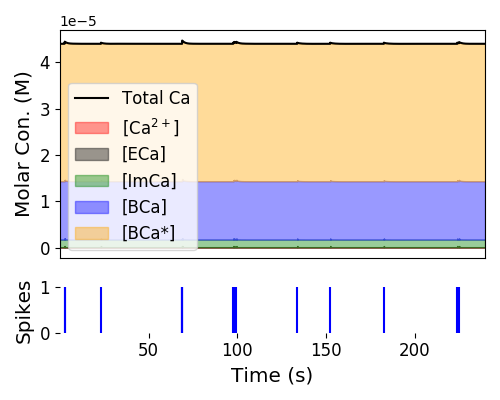
\includegraphics[width=\textwidth]{figures/concentration_dynamics_18.png}
    \caption{}
    \label{fig:concentration_dynamics_a}
  \end{subfigure}
  \begin{subfigure}{0.5\textwidth}
    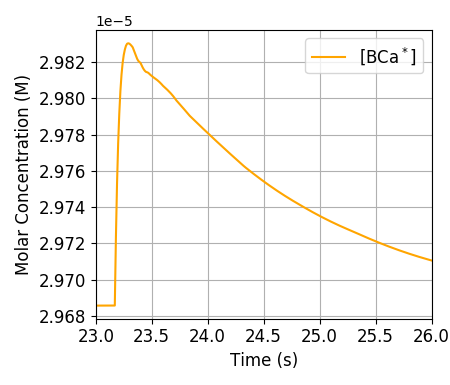
\includegraphics[width=\textwidth]{figures/concentration_dynamics_18_zoomed_BCa_star.png}
    \caption{}
  \end{subfigure}
  \begin{subfigure}{0.5\textwidth}
    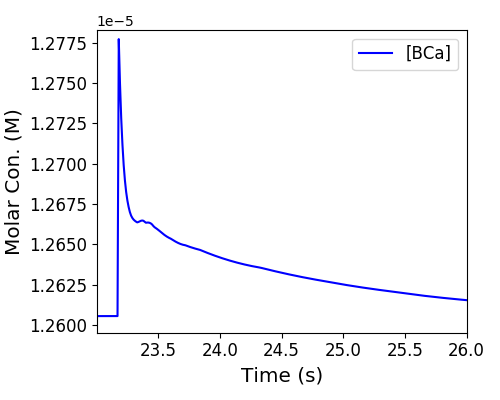
\includegraphics[width=\textwidth]{figures/concentration_dynamics_18_zoomed_BCa.png}
    \caption{}
  \end{subfigure}
  \begin{subfigure}{0.5\textwidth}
    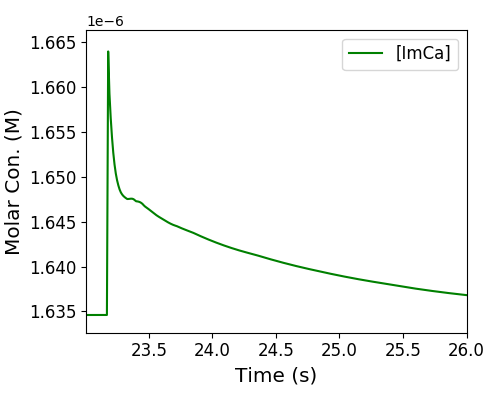
\includegraphics[width=\textwidth]{figures/concentration_dynamics_18_zoomed_ImCa.png}
    \caption{}
  \end{subfigure}
  \begin{subfigure}{0.5\textwidth}
    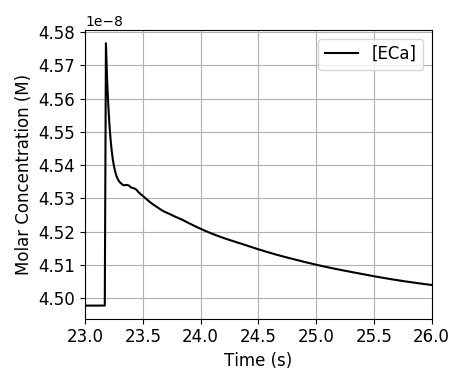
\includegraphics[width=\textwidth]{figures/concentration_dynamics_18_zoomed_ECa.png}
    \caption{}
  \end{subfigure}
  \begin{subfigure}{0.5\textwidth}
    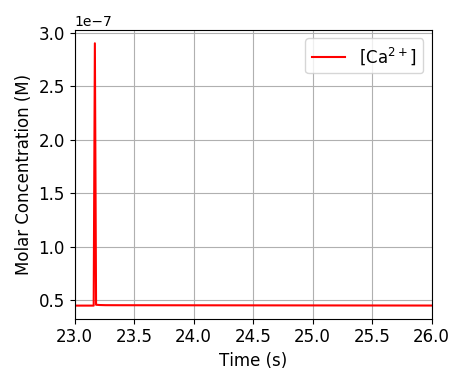
\includegraphics[width=\textwidth]{figures/concentration_dynamics_18_zoomed_Ca.png}
    \caption{}
  \end{subfigure}
  \caption{\textbf{Calcium Buffering Dynamics } (a) The proportions of bound and free calcium concentrations within a cell, with the associated spike train. (b)-(f) The dynamics of the concentration of (b) excited indicator bound calcium, (c) indicator bound calcium, (d) immobile endogenous buffer bound calcium, (e) mobile endogenous buffer bound calcium, and (f) free calcium in response to an action potential at $\sim$23.2s.}
  \label{fig:concentrations}
\end{figure}

% (New Figure 3X (Insert more commentary on this once the new figure is added))

When calcium entered the model neuron it was rapidly buffered \cite{bartol}. However the relative fractions of which buffer molecules bound to the influxed calcium was dynamic, and changed over time . Figure \ref{fig:concentrations} (b-f) shows the time course of the various species over time in response to a calcium influx event from a single action potential. Crucially, the indicator $[BCa]$ competed with the endogenous buffers $[ImCa]$ and $[ECa]$ – all three bind calcium on similar timescales. This implies that the timecourse and amplitude of the $[BCa]$ variable will also depend on the binding rates and availabilities of the endogenous buffers. For example if we decreased the concentration of an endogenous buffer, we might expect both a faster rise time and greater peak amplitude of the $[BCa]$ signal in response to a calcium influx event. The slowest component of the decay had a similar time constant for $[BCa]$, $[ImCa]$ and $[ECa]$, which in turn matched the $[Ca]$ extrusion time constant in our model ($\sim 6.29 \times 10^{-22}$Ms$^{-1}$). This implies that the buffers and the indicator had reached a dynamic equilibrium and were jointly tracking the free calcium concentration as calcium was slowly extruded from the cell.

Interestingly the excited bound calcium species ($[BCa^*]$) showed a qualitatively different timecourse in response to a calcium influx event. This concentration is subject to the added `excitation and release' dynamic, where a certain proportion of the concentration absorbs the energy from an incoming photon and goes into an `excited state' at each time step. A certain proportion of the concentration releases a photon and reverts to a `relaxed state' at each timestep also. This means that the excited bound calcium lags behind the bound calcium trace. We could think of the excited bound calcium trace as a low pass filtered version of the bound calcium trace.

\subsection{Spike inference accuracy is sensitive to indicator properties, and likely varies within and between cells}
The above results imply that the fluorescence signal depends on the relative properties of both GCaMP and the endogenous buffers. We next used the model to directly ask how sensitive spike inference was to these components. We focused on three key parameters that likely vary from cell to cell and experiment to experiment: GCaMP binding kinetics, GCaMP concentration, and endogenous buffer concentration.

Several variants of GCaMP itself have been made that differ in calcium binding kinetics, baseline fluorescence, fluorescence efficiency, and other factors. For example, GCaMP6f has a decay time constant of $\sim 1$s, while GCaMP6s has a decay time constant of $\sim 2$s \cite{chen}. Here we asked how these differences in binding kinetics affect spike inference. We jointly varied the calcium binding and unbinding rates of the indicator by the same factor over a range from $100$-fold slower to $100$-fold faster from the fitted values, and simulated the fluorescence response for each of the parameter settings in response to the same spike trains as before (figure \ref{fig:rates_perturbed}). Notably this manipulation does not affect the indicators affinity, and therefore would not affect steady-state responses to prolonged changes in calcium. Instead it is likely to affect its sensitivity to the spike train dynamics. We computed two summary measures from the simulated fluorescence traces: the signal-to-noise ratio for a single spike (Methods, section \ref{sec:snr}), and the accuracy of spike inference for each of the spike trains. We observed a reduction in the signal-to-noise ratio and the spike inference quality when we set the binding and unbinding rates were set to one hundreth of their fitted values, and to one tenth of their fitted values. When we increased the value of both binding rates, we observed no change in these measurements. The reduction in both rates lead to smaller increases in fluorescence in response to an action potential and a longer decay time (figure \ref{fig:rates_perturbed_fluorescence}), this caused the reduction in signal-to-noise ratio. As both rates were increased, the change in $\Delta F/F_0$ in response to an action potential increased and the decay time decreased slightly, but the fluorescence trace created by these values was very similar to the trace created by the fitted values.

\begin{figure}[p]
\centering
    \begin{subfigure}{0.9\textwidth}
        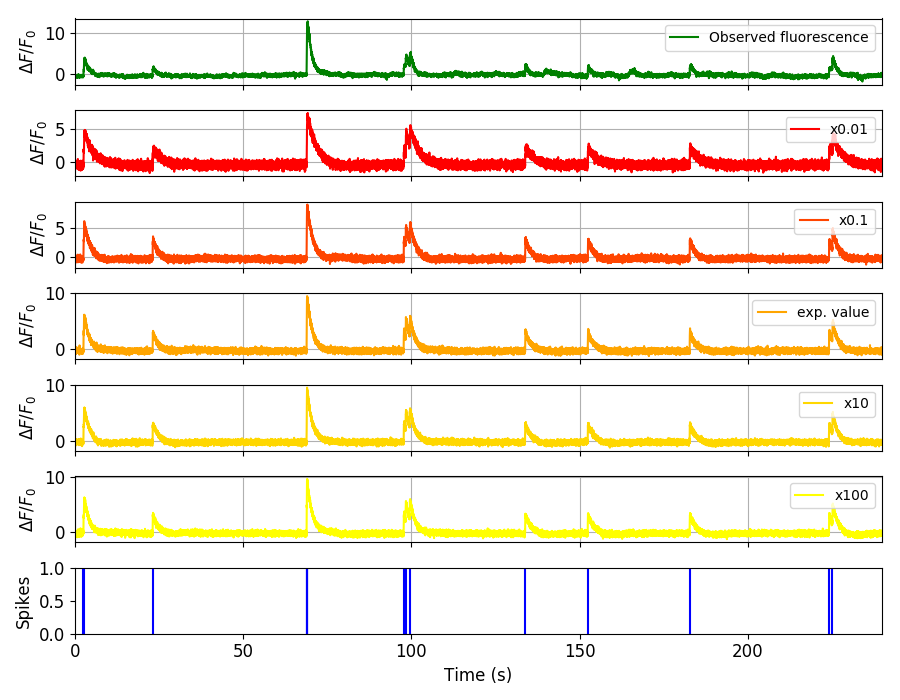
\includegraphics[width=\linewidth]{figures/b_i_f_i_perturbed_fluorescence_18_paper.png}
        \caption{}
        \label{fig:rates_perturbed_fluorescence}
    \end{subfigure}
    \newline
    \begin{subfigure}{0.45\textwidth}
        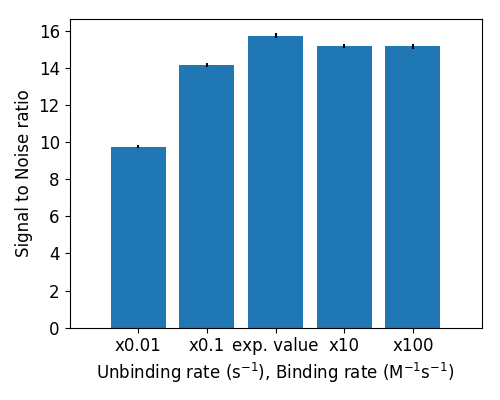
\includegraphics[width=\linewidth]{figures/b_i_f_i_perturbed_snr.png}
        \caption{}
        \label{fig:rates_perturbed_snr}
    \end{subfigure}
    \begin{subfigure}{0.45\textwidth}
        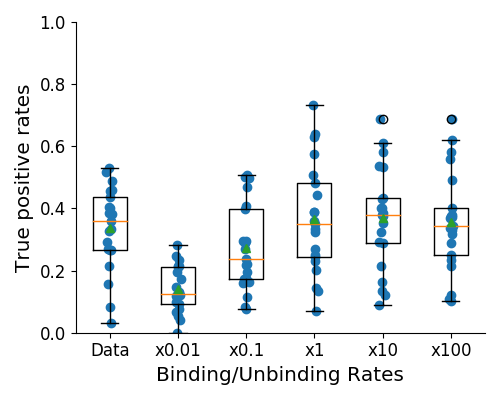
\includegraphics[width=\linewidth]{figures/b_i_f_i_perturbed_oasis_tp_paper.png}
        \caption{}
        \label{fig:rates_perturbed_inference}
    \end{subfigure}
    \caption{(a) An example trace for each of the five pairs of values used for the binding and unbinding rates of the fluorescent calcium indicator. (b) The signal-to-noise ratio of the modelled fluorescence traces using each of the four perturbed values, and the experimental value. The SNRs for the two pairs with values lower than the experimental value are lower than the experimental pair or the higher value pairs. (c) The true-positive rates of the deconvolution algorithm's predictions when inferring from the observed data, and inferring from modelled traces using the perturbed and experimental values.}
    \label{fig:rates_perturbed}
\end{figure}

\begin{figure}[p]
    \centering
    \begin{subfigure}{0.9\textwidth}
        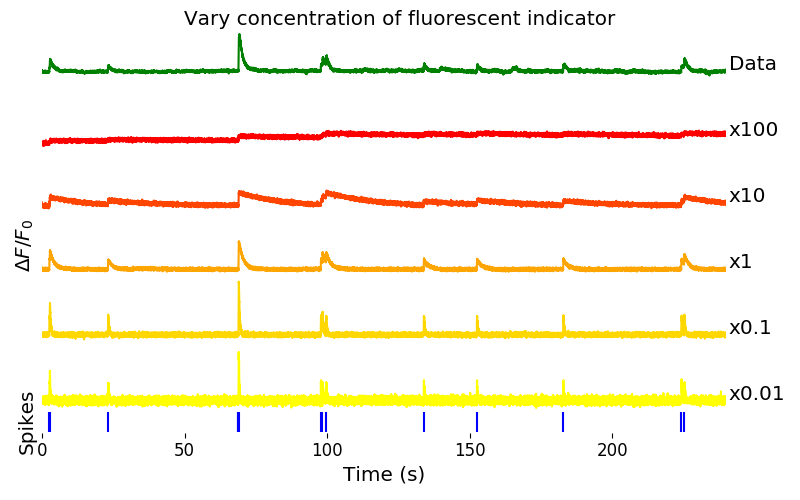
\includegraphics[width=\linewidth]{figures/indicator_perturbed_fluorescence_18_paper.png}
        \caption{}
        \label{fig:indicator_perturbed_fluorescence}
    \end{subfigure}
    \newline
    \begin{subfigure}{0.45\textwidth}
        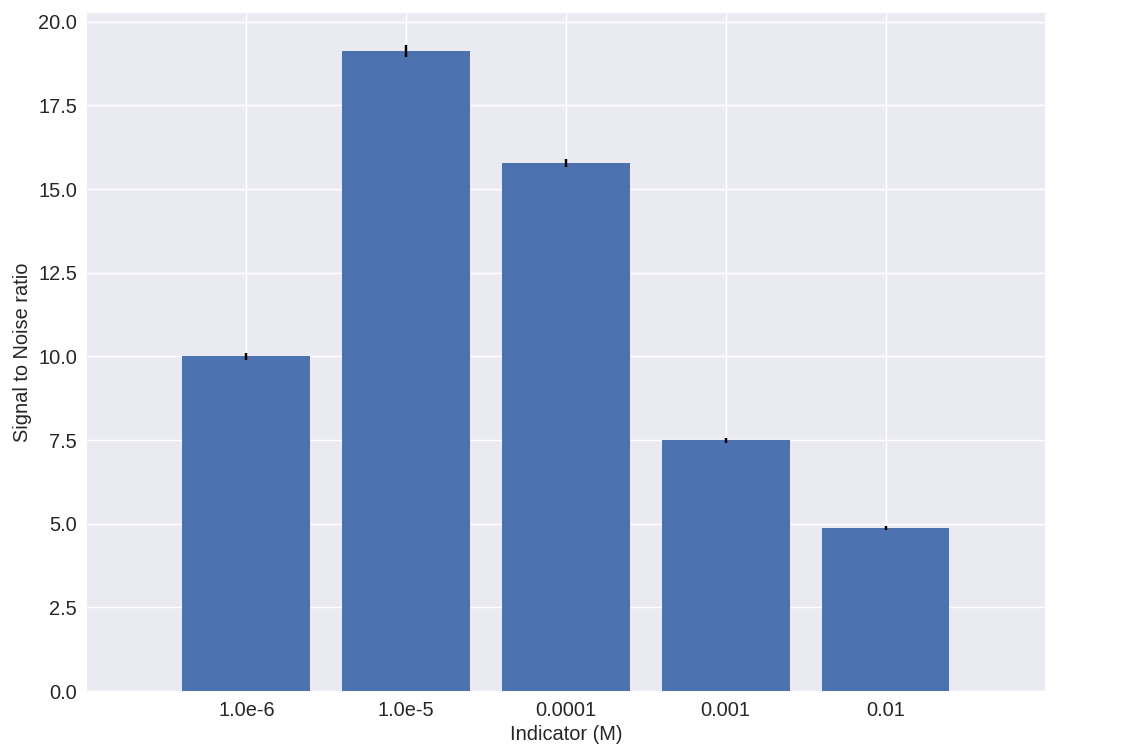
\includegraphics[width=\linewidth]{figures/indicator_perturbed_snr.png}
        \caption{}
        \label{fig:indicator_perturbed_snr}
    \end{subfigure}
    \begin{subfigure}{0.45\textwidth}
        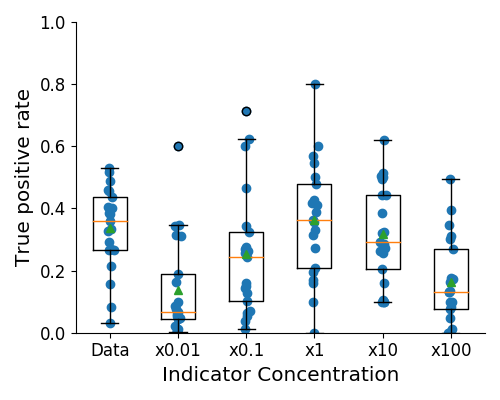
\includegraphics[width=\linewidth]{figures/indictor_perturbed_oasis_first_paper.png}
        \caption{}
        \label{fig:indicator_perturbed_inference}
    \end{subfigure}
    \caption{(a) An example trace for each of the five perturbed values for the concentration of fluorescent calcium indicator. The top two traces are produced by the lower perturbed values, the middle trace is produced by the experimental value, and the lowest two traces are produced when using the higher perturbed values. (b) The signal-to-noise ratio of the modelled fluorescence traces using each of the four perturbed values, and the experimental value. Extreme perturbations of the concentration either above or below the experimental level lowered the SNR. (c) The true-positive rates of the deconvolution algorithm's predictions when inferring from the observed data, and inferring from modelled traces using the perturbed and experimental values. We found that the algorithms performs equally badly on the two most extreme values, and performs equally well on the experimental value, and the next higher perturbed value.}
    \label{fig:indicator_perturbed}
\end{figure}

Second, the overall concentrations of GCaMP often varies from cell to cell. For example different cells, even of the same type in the same tissue, can express different levels of GCaMP, due to proximity to the infection site, or the cell becoming `nuclear-filled'\cite{tian, chen}. Also, GCaMP is often used for longitudinal experiments where the same cells are re-imaged across multiple days or weeks. However since GCaMP expression typically ramps up over time \cite{chen}, the accuracy of spike inference may differ across multiple longitudinal recordings in the same cell. We addressed this by varying the concentration of calcium indicator in the model, simulating spike trains and measuring signal-to-noise ratio and spike inference accuracy on the resulting fluorescence traces. Both increasing and decreasing the concentration of the indicator had effects on the fluorescence trace, signal-to-noise ratio, and spike inference. The signal-to-noise ratio and spike inference quality decreased with decreased indicator concentration, and both showed a decrease when the indicator concentration was increased to $100$ times it's fitted value (figure \ref{fig:indicator_perturbed}). The signal-to-noise ratio showed an increase when the indicator concentration was increased to $10$ times it's fitted value, but there was no corresponding change in the spike inference quality. The decrease in indicator concentration caused a reduction in the increase in $\Delta F/F_0$ in response to an action potential, and an increase in the decay time of this increase (figure \ref{fig:indicator_perturbed_fluorescence}). The increase in indicator concentration had the opposite effect, it casued an increase in the change in $\Delta F/F_0$ in response to an action potential, and a decrease in the decay time.

Third, the concentration and types of endogenous calcium buffers also vary from neuron to neuron, both within and between cell types\cite{bartol, maravall, neher}. Since the calcium buffer capacity of neurons is high, around 50-70\cite{lee} in excitatory hippocampal pyramidal cells, around 100-250\cite{lee} in inhibitory hippocampal pyramidal cells, and 900-200 in Purkinje cells (depending on the age of the subject), these endogenous buffers compete with GCaMP for binding to calcium, and variations in endogenous buffer concentration may affect GCaMP signal and therefore spike inference. To address this we varied the concentration of the endogenous buffer in the model neuron over five orders of magnitude from $0.8$ to $8000$ $\mu$M, simulated calcium fluorescence traces in response to the same set of spike trains, and performed spike inference on the resulting fluorescence time series. Increasing the endogenous buffer concentration had a substantial effect on the GCaMP fluorescence signal, both decreasing its amplitude and slowing its kinetics (figure \ref{fig:endogenous_perturbed}(a)). This corresponded with a decrease in both single-spike signal-to-noise ratio (figure \ref{fig:endogenous_perturbed}(b)) and spike inference accuracy (figure \ref{fig:endogenous_perturbed}(c)). In contrast, decreasing endogenous buffer capacity from the fitted value had little effect on either the GCaMP signal or spike inference (figure \ref{fig:endogenous_perturbed}).

\begin{figure}[p]
    \centering
    \begin{subfigure}{0.9\textwidth}
        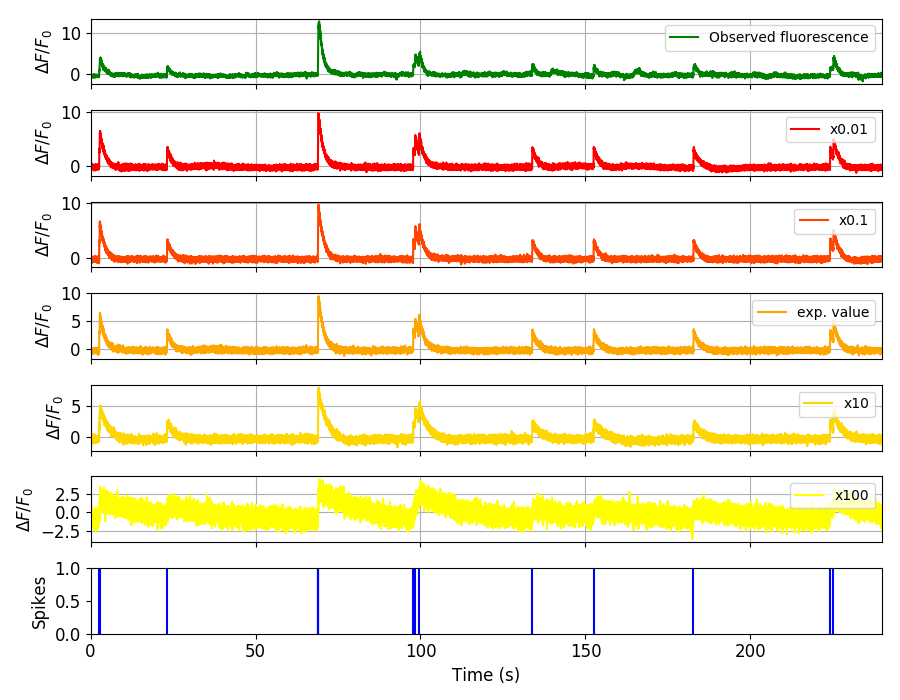
\includegraphics[width=\linewidth]{figures/immobile_perturbed_fluorescence_18_paper.png}
        \caption{}
    \end{subfigure}
    \newline
    \begin{subfigure}{0.45\textwidth}
        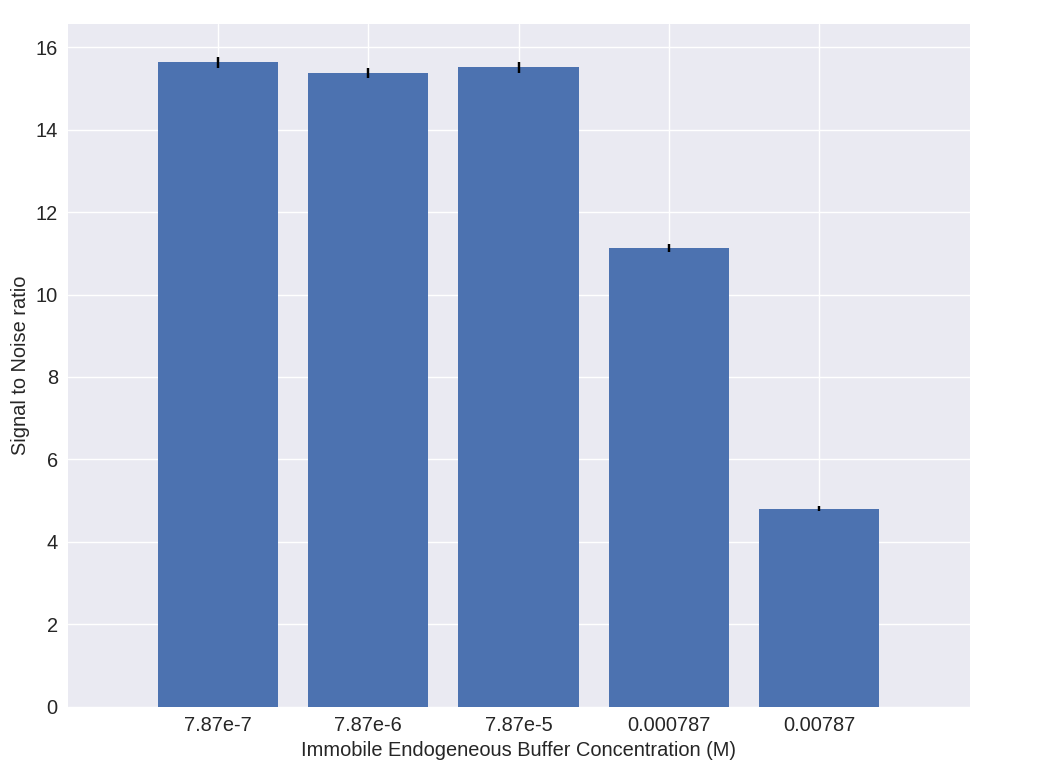
\includegraphics[width=\linewidth]{figures/immobile_perturbed_snr.png}
        \caption{}
    \end{subfigure}
    \begin{subfigure}{0.45\textwidth}
        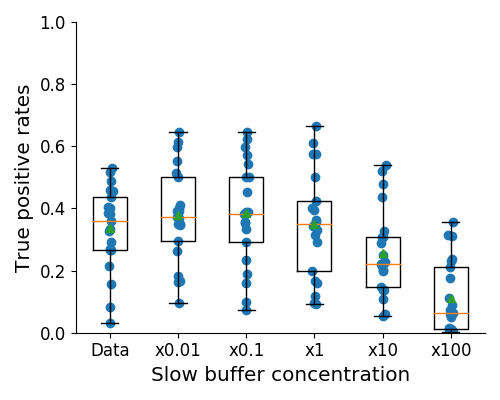
\includegraphics[width=\linewidth]{figures/immobile_perturbed_oasis_first_paper.png}
        \caption{}
    \end{subfigure}
    \caption{(a) An example trace for each of the five perturbed values for the concentration of immobile endogenous buffer.	(b) The signal-to-noise ratio of the modelled fluorescence traces using each of the four perturbed values, and the experimental value. The lower values for the immobile buffer produce the same SNR as the experimental value. But the higher perturbed values produce fluorescence traces with a lower SNR.	(c) The true-positive rates of the deconvolution algorithm's predictions when inferring from the observed data, and inferring from modelled traces using the perturbed and experimental values.}
    \label{fig:endogenous_perturbed}
\end{figure}

\subsection{Single spike inference accuracy drops for high firing rates, but firing rate itself can be estimated from mean fluorescence amplitude}
The fluorescence signal recorded from neurons using calcium indicators is typically much slower than changes in membrane potential for two reasons: first, because the calcium and the indicator have slow binding and unbinding kinetics, the signal is a low-pass filtered version of the membrane potential. Second, neuronal two-photon imaging experiments are often performed in scanning mode, which limits their frame rate to $\sim 10$Hz or slower. This implies that multiple spike events that occur close in time might be difficult to resolve from a calcium indicator time series. Many cells, especially several types of inhibitory interneurons, fire tonically at rates higher than $10$Hz. We used the model to test whether spike inference accuracy depended on the neuron’s firing frequency by driving the cell with spike trains sampled from a Poisson processes of varying frequency. We simulated a variable firing rate using an Ornstein-Uhlenbeck process, and simulated the spike trains using a Poisson distribution with its rate taken from this process. Because of the high frequency firing rate of these spike trains, we using the accuracy as the measure of spike inference quality. We simulated $30$ spike trains at average firing rate of $1$, $5$, and $10$Hz, and measured the spike inference quality of all these traces. Spike inference accuracy decreased with increasing firing rate, for up to $10$Hz Poisson spike trains (figure \ref{fig:frequency_comparison_measures}(left)). Although, the accuracy remained above $90\%$ for each of the three frequencies. We also plotted the average $\Delta F/F_0$ as a function of stimulation firing rate. We found that it increased monotonically as a function of firing rate (figure \ref{fig:frequency_comparison_measures}(right)).

We expected lower spike inference quality as the average spiking frequency increased. Since the fluorescence trace, in some sense, is a low pass filtered version of the spike train, a tightly packed groups of spikes will be more difficult to infer than isolated spikes. However, the increasing amplitude of the fluorescence trace with increasing frequency suggests that some spike inference algorithm could be developed based on this amplitude.

\begin{figure}[h]
  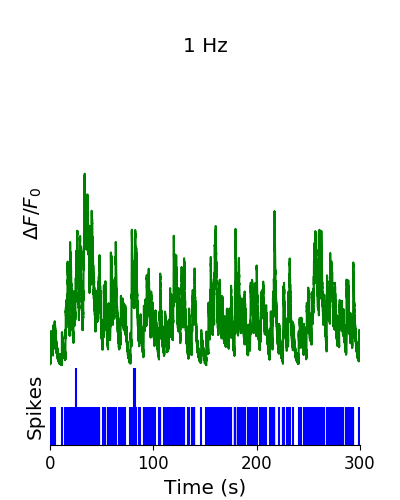
\includegraphics[width=0.329\linewidth]{figures/paper_fig_1_Hz_1_3.png}
  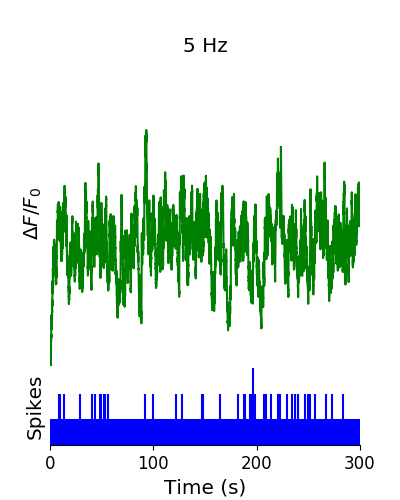
\includegraphics[width=0.329\linewidth]{figures/paper_fig_5_Hz_1_2.png}
  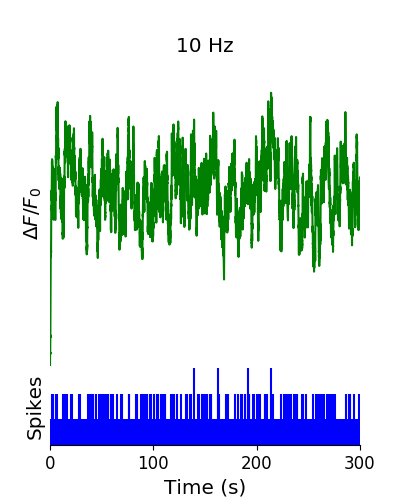
\includegraphics[width=0.329\linewidth]{figures/paper_fig_10_Hz_1_1.png}
  \caption{\textbf{Simulating fluorescence traces at different firing rates } Example modelled traces created using simulated spike trains with a mean firing rate of $1$Hz (left column), $5$Hz (middle column), and $10$Hz (right column). Note the difference in amplitude with different mean firing rates.}
  \label{fig:frequency_comparison_traces}
\end{figure}

\begin{figure}[h]
\centering
  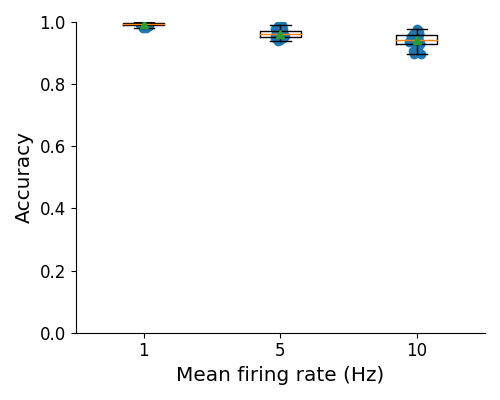
\includegraphics[width=0.45\linewidth]{figures/simulated_oasis_accuracy_paper.png}
  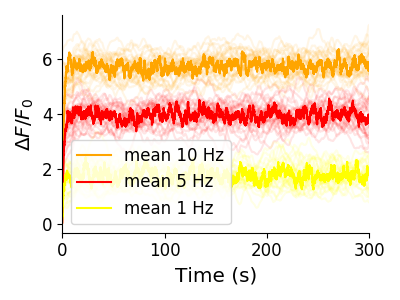
\includegraphics[width=0.45\linewidth]{figures/mean_fluorescence_comparison.png}
  \caption{\textbf{Inference quality and $\Delta F/F_0$ vs Firing rate} (left) The spike inference accuracy when applied to 30 traces created using simulated spike trains with mean firing rates of 1, 5, and 10 Hz. (right) The mean $\Delta F/F_0$ across those 30 traces for each frequency.}
  \label{fig:frequency_comparison_measures}
\end{figure}

\section{Discussion}
We designed a biophysical model for the changes in free calcium and bound calcium concentrations within a cell soma with a fluorescent calcium indicator. We used this model to model the fluorescence trace resulting from a spike train in this cell.  We fit the free parameters of the model by matching the power spectrum and amplitude of fluorescence traces with simultaneously measured spike trains. We inferred spikes from real fluorescence traces and modelled fluorescence traces, and measured the quality of the spike inference in both cases. We found that the spike inference quality was similar in both cases. We perturbed the concentration of the calcium buffers in the model, and the binding/unbinding rates of those buffers in the model, and measured the effect on the signal-to-noise ratio (SNR) of the modelled fluorescence traces and the spike inference quality.

For the fluorescent calcium indicator, we found that any large perturbation away from the experimental value led to a reduction in SNR, and spike inference quality. For the binding/unbinding rates, we kept the ratio of these rates constant, but altered their values in parallel. The lower values caused a reduction in SNR, and a reduction in spike inference quality. For the endogenous buffer concentration, an increase above the experimental value caused a reduction in SNR and spike inference quality.

Although the model produced visually similar time series to the real data, there were a few aspects it did not capture. First, the real data featured some low-frequency components that did not appear related to the spike events. These were not captured by the models we used in this study, but could be added in future by adding a suitable low-frequency term to the resulting time series. Second, the real data seemed to have some nonlinearities not captured in the model, for example the response to two nearby spikes was greater than expected from the linear sum of two single spikes. This may be due to the co-operative binding of Calmodulin to calcium, which gives calmodulin a supra-linear sensitivity to calcium concentration. The model, in contrast behaved much more linearly, but could be extended in future to include such nonlinearities. Third, in the real data the fluorescence peak amplitude seemed to vary from spike to spike, even for well-isolated spike events. However in our model we assumed each spike lead to the same fixed-amplitude injection of calcium to the cell, leading to much greater regularity in fluorescence peak amplitudes. This variability could be added in future versions of the model by making the injected calcium peak a random variable. Fourth, we modelled the soma as a single compartment, but in reality there is likely a non-uniform spatial profile of calcium concentration. This may matter because some endogenous buffers might access calcium right as it influxes from the extracellular space, whereas the majority of the fluorescence signal is more likely coming from the bulk of the cytoplasm. Future models could attempt to model these spatial dependencies to assess whether they affect the overall spike inference procedure.

As well as the optimised parameters, the model has 14 fixed parameters than can be changed to simulate different types of calcium indicators. This model could be used to test the theoretical performance of proposed new types of calcium indicator. The model could also be used by developers of spike inference algorithms to test the effects of changing calcium indicator parameters on spike inference, or to test the affects of changing spiking characteristics on spike inference. For example, high firing rate vs low firing rate, or bursting vs no bursting. Given the increasing amplitude of the fluorescence trace with increasing mean firing rate, it would be possible to build a spike inference algorithm on this principle at least in part.

Our model has already been used as a tool by our colleagues, for simulating fluorescence traces in response to cells that can fire with a continuous rate between $10$ and $20$Hz, but do not always do so. Our colleagues found that a combination of the amplitude and the variance of the simulated fluorescence trace was the best indicator of firing rate. For example, when a cell was not firing, the amplitude and variance of the fluorescence trace was relatively low. When the cell fired with a low firing rate $\sim 1$Hz, the mean amplitude was still low but the variance of the fluorescence trace was high, and for high firing rate $\sim 10-20$Hz, the fluorescence amplitude was high, and the variance was low. In this way, our model may be useful for investigating firing rates underlying real fluorescence traces in response to cells which can fire in these rage ranges.

A recent paper by Greenberg et al (2018) described a biophysical model for spike train inference called the `Sequential binding model'. Similar to our model, this model included parameters for two types of endogenous buffer. But this model also included dynamics for calcium binding to and unbinding from these endogenous buffers. Furthermore, this model included dynamics for calcium binding to and unbinding from the four binding sites present on a GCaMPs6 molecule. In the accuracy measurements specified in that paper, this model performed better than the MLspike algorithm, which is also partially a biophysically model, and it performed better than the constrained non-negative deconvolution algorithm. The sequential binding model also biophysically interpretable parameters, and its fitted parameters for quantites such as buffering capacity and calcium influx upon action potential firing fall in line with experimental values\cite{greenberg}. Biophysical models like this appear to be the way forward for spike inference algorithms.

\section{Methods}
\subsection{Calcium dynamics model}
We wrote a biophysical model of the calcium dynamics within a cell soma. When a neuron fires an action potential, voltage-dependent calcium ion-channels open up that allow a current of Ca$^{2+}$ to flow into the neuron \cite{koch}. The increase in the free calcium ion concentration inside of the cell, along with changes in the concentration of potassium and sodium, causes the change in cell membrane potential, which must be depolarised. The depolarising process consists of free calcium ions leaving the cell through open ion channels, or binding to molecules within the cell called buffers, or calcium storage by organelles such as the endoplasmic reticulum. A diagram illustrating the cell, its channels, and its buffers can be seen in figure \ref{fig:spike_finder_example}A. There are several different types of calcium buffer, each with different dynamics and different concentrations within different types of excitable cell. The fluorescent calcium indicator is another calcium buffer, with the useful property that when it is bound to a calcium ion, the bound molecule may become excited by a photon and release a photon in return. This is what creates the fluorescence. After the action potential has taken place, the free calcium concentration within the cell will return to a baseline level \cite{maravall}.

We modelled the the dynamics of five molecular concentrations,
\begin{itemize}
    \item Free calcium ion concentration, $[Ca^{2+}]$
    \item Fluorescent indicator bound calcium, $[BCa]$
    \item Endogenous mobile buffer bound calcium, $[ECa]$
    \item Endogenous immobile buffer bound calcium, $[ImCa]$
    \item Excited buffered calcium, $[BCa^{\ast}]$
\end{itemize}
The term ‘buffering’ refers to free calcium ions coming into contact with buffer molecules and binding together. Diagrammatically:
\begin{align*}
    [X][Ca^{2+}] \xrightleftharpoons[k_{Xb}]{k_{Xf}} [XCa]
\end{align*}
where $[X]$ represents any buffer molecule, and $k_{X_f}$ and $k_{X_b}$ represent the binding and unbinding (dissociation) rates in units of per molar concentration per second (M$^{−1}$ s$^{−1}$) and per second (s$^{−1}$) respectively. The speed of this chemical reaction is determined by the binding and unbinding rates.

There are a number different endogenous buffers in any neuron. Which buffers are present, and the buffers’ concentrations vary from cell to cell. In order to capture the effects of mobile and immobile endogenous buffers without introducing several parameters, they were modelled as two buffers. One representing mobile buffers and the other representing immobile buffers. Each with their own binding and unbinding rates.

The fluorescent calcium indicator behaves similarly to the other calcium buffers. The calcium is buffered by the indicator in the same way. But an indicator bound calcium molecule can become excited by absorbing the energy from a photon. An excited indicator bound calcium molecule can then release a photon to go back to its ‘relaxed’ state.
\begin{align*}
    [B][Ca^{2+}] \xrightleftharpoons[k_{Bb}]{k_{Bf}} [BCa] \leftrightsquigarrow [BCa^{\ast}]
\end{align*}
The released photons are captured by a photon collector. This gives us the fluorescence trace.

Ignoring the baseline level of free calcium in a neuron, the system of equations we used to model all of these interactions is as follows:
\begin{equation} \label{eq:model_equations}
  \begin{split}
  \diff{[Ca^{2+}]}{t} = & k_{Bb}[BCa] + k_{Eb}[ECa] + k_{Imb}[ImCa] \\
                      & - k_{Bf}[B][Ca^{2+}]- k_{Ef} [E][Ca^{2+}] - k_{Imf}[Im][Ca^{2+}] \\
                      & + \beta ([Ca^{2+}_{0}] - [Ca^{2+}])
  \end{split}
\end{equation}
\begin{align}
  \diff{[BCa]}{t} = & k_{Bf}[B][Ca^{2+}] - k_{Bb}[BCa] + r[BCa^{*}] - e[BCa] \\
  \diff{[ECa]}{t} = & k_{Ef}[E][Ca^{2+}] - k_{Eb}[ECa] \\
  \diff{[ImCa]}{t} = & k_{Imf}[Im][Ca^{2+}] - k_{Imb}[ImCa] \\
  \diff{[BCa^{*}]}{t} = & \eta[BCa] - r[BCa^{*}]
\end{align}
where $[Ca^{2+}_{0}$ is the baseline calcium concentration within the cell soma, $\beta$ is a rate defining how quickly free calcium enters or leaves the cell in the absence of an action potential, $\eta$ is the excitation rate for indicator bound calcium, r is the photon release rate for the excited indicator bound calcium, and f and b are used to indicate the forward and backward rates for chemical reactions respectively. The excitation rate defines the proportion of indicator bound calcium that becomes excited at each time step. The photon release rate defines the proportion of excited indicator bound calcium that releases a photon and returns to its relaxed state at each time step. An action potential is modelled as a discontinuous increase in the free calcium concentration to an appropriate value \cite{maravall}.

Note that each of the three pairs of binding and unbinding terms in the first equation has a corresponding pair in one of the subsequent three equations. Binding removes a free calcium molecule and adds a bound calcium molecule, and unbinding does the opposite.

When using this model to simulate a fluorescence trace, the system of equations above are first solved over a period of 25s without action potentials. This lets each of the five tracked chemical concentrations reach their steady state. Then we use the given spike train and the parameters to model the fluorescence trace.

Note that since the model has no spatial component, the mobile and immobile buffers only differ in their binding and unbinding rates.

\subsubsection{Photon release \& capture}
We used a simple model for the photon release. The number of photons released at each time step was controlled by the number of excited indicator bound calcium molecules in the cell and a parameter called the `release rate'. The release rate is an optimised free parameter of the model.

As for the photon capture, in two-photon excitation microscopy the photons scattered by the fluorescent indicator get scattered in all directions. Therefore the number of photons detected is stochastic. This made the process for capturing photons the natural source of noise in the system. The number of photons captured, and therefore the intensity of the fluorescence, is modelled using a binomial distribution. The number of photons released was used as the number of trials. The probability of success, or `capture rate' was a free parameter of the model that we optimised.

\subsection{Parameter optimisation}\label{sec:parameter_optimisation}
The free parameters of the model are as follows:
\begin{description}
    \item[Calcium rate, $\beta$] Controls how quickly the concentration of free calcium will be driven to the baseline concentration.
    \item[Capture rate, $p$] The average proportion of photons captured by the photon detector.
    \item[Excitation rate, $\eta$] The number of indicator bound calcium molecules that become excited by photon bombardment at each time step.
    \item[Release rate, $r$] The number of excited indicator bound calcium molecules that release a photon at each time step.
\end{description}
To optimise the free parameters given a fluorescence trace, we applied the following procedure:
\begin{enumerate}
    \item The frequency power spectrum of the trace was measured.
    \item The power spectrum was smoothed using a boxcar smoother (aka. sliding average, box smoother).
    \item The log of the smoothed power spectrum was measured.
    \item Use the model to create a modelled fluorescence trace.
    \item Apply steps 1, 2, and 3 to the modelled fluorescence trace.
    \item Calculate the root mean squared difference between the log power of the actual fluorescence trace, and the log power of the modelled fluorescence trace.
    \item Calculate the root mean squared difference between the actual fluorescence trace and the modelled fluorescence trace.
    \item Use an optimisation algorithm to reapply this process, attempting to minimize the sum of the two root mean squared differences at each iteration.
\end{enumerate}
Using the root mean squared difference of the log power spectra as part of the objective function forces the model to match the noise frequency of the actual fluorescence. Using the root mean squared difference of the traces themselves forces the model to match the amplitude of the fluorescence trace more accurately.

In order to minimise the objective function, a suite of meta-heuristic optimisation (aka. black-box optimisation) algorithms were implemented on each of the traces in the dataset. These methods were chosen because they don’t require a gradient for the objective function (gradient-free) and they are particularly useful for minimising stochastic objective functions like the one we used here. The free parameters were optimised for each individual fluorescence trace. The most successful method for each trace was recorded. The method that was most often successful was probabilistic descent, and the second most successful method was generating set search. Both of these methods are examples of pattern search. These two methods were the best optimisers on about $75\%$ of the traces in the dataset.

Although this optimisation procedure minimises the value of the optimisation function, the value never reaches zero for a number of reasons. Firstly, the fluorescence traces carry low frequency fluctuations that cannot be captured by the model. Secondly, the model assumes that the process of calcium binding to the fluorescent indicator is linear in time (see equation 1), but there are more complicated dynamics involved here. Fluorescent calcium indicators are often built upon the calcium binding protein called `calmodulin'. This protein has four calcium binding sites. These sites are locally split into two pairs. Each pair has a different affinity for calcium, and the affinity of the binding sites is affected by the occupancy of the other binding sites \cite{kilhoffer}. So the calcium to calcium indicator binding process is non-linear, but the model does not take this into account.

\subsubsection{Fixed parameters}
As well as the optimised parameters mentioned in section \ref{sec:parameter_optimisation}, the model also has thirteen fixed parameters. Please see table \ref{tab:fixed_parameters} for details of these parameters and their values. In an application of the model, these parameters can be changed in order to model any given fluorescent calcium indicator.

\begin{table}
    \centering
    \begin{tabular}[t]{|l|p{6cm}|c|c|}
        \hline
        \textbf{Parameter}  & \textbf{Description}                                                                      & \textbf{Value}                        & \textbf{Source} \\ \hline
        baseline            & The baseline concentration of free calcium within the cell soma                           & $4.5 \times 10^{−8}$M                 & \cite{maravall} \\ \hline
        cell radius         & The radius of the soma (assumed to be spherical)                                          & $10^{-5}$M                            & \cite{fiala} \\ \hline
        endogenous         & The concentration of endogenous mobile buffer within the cell soma                       & $10^{-4}$M                            & \cite{faas} \\ \hline
        frequency           & The frequency at which the spike trains are sampled.                                      & $100$Hz                               & \\ \hline
        immobile            & The concentration of endogenous immobile buffer within the cell soma                     & $7.87 \times 10^{-5}$M                & \cite{bartol} \\ \hline
        indicator           & The concentration of fluorescent indicator within the cell soma                           & $10^{-4}$M                            & \cite{maravall} \\ \hline
        $k_{Bb}$            & The unbinding rate of the fluorescent calcium indicator                                   & $160s^{−1}$                           & \cite{bartol} \\ \hline
        $k_{Bf}$            & The binding rate of the fluorescent calcium indicator                                     & $7.77 \times 108$s$^{−1}$M$^{−1}$     & \cite{bartol} \\ \hline
        $k_{Eb}$            & The unbinding rate of the endogenous mobile buffer                                       & $10^4$s$^{-1}$                        & \cite{bartol} \\ \hline
        $k_{ef}$            & The binding rate of the endogenous mobile buffer                                         & $10^8$s$^{-1}$M$^{-1}$                & \cite{bartol} \\ \hline
        $k_{Imb}$           & The unbinding rate of the endogenous immobile buffer                                     & $524$s$^{-1}$                         & \cite{bartol} \\ \hline
        $k_{Imf}$           & The binding rate of the endogenous immobile buffer                                       & $2.47 \times 10^{8}$s$^{-1}$M$^{-1}$  & \cite{bartol} \\ \hline
        peak                & The increase in free calcium concentration within the cell induced by an action potential & $2.9 \times 10^{-7}$M                 & \cite{maravall} \\ \hline
    \end{tabular}
    \caption{\textbf{Fixed parameters} A table of the parameters fixed before optimising the model. The values of these parameters could be changed to model different fluorescent calcium indicators.}
    \label{tab:fixed_parameters}
\end{table}

\subsection{Julia}
The programming language used to write and execute the model was `Julia'. Julia is a dynamic programming language designed for technical computing. Julia was designed specifically to provide a convenient high-level dynamic language similar to MATLAB, or Python, with improved performance. Julia's type system and Julia’s direct interfaces with C and Fortran allow this aim to be achieved \cite{bezanson}. The Julia version of the `Sundials' package for ODE solving was used to solve the system of equations above. The \texttt{BlackBoxOptim.jl} package for Julia was used to perform the optimisation.

\subsection{Spike inference}
We used spike inference algorithms to compare the quality of spike inference using the modelled traces to the quality of spike inference using the observed traces. We also used the spike inference algorithms to assess the effect of parameter perturbation on the spike inference. Three algorithms were used:
\begin{description}
    \item[Constrained non-negative deconvolution algorithm (aka Pnevmatikakis algorithm)] This algorithm uses a constrained version of non-negative Weiner deconvolution to infer a calcium signal and a `spiking activity signal' from the fluorescence trace \cite{vogelstein, pnevmatikakis}. The spiking activity signal is a non-negative vector of real numbers reflecting the cell's activity rather than an actual spike train. We inferred a spike train by choosing an optimised threshold for the spiking activity signal. Whenever the spiking activity signal exceeded that threshold, an action potential was inferred. The threshold was optimised by minimising the difference between the number of spikes observed and the number of spikes predicted.
    \item[ML-Spike algorithm] This algorithm uses a generalised version of the Viterbi algorithm to return the spike train that maximises the likelihood of producing the given fluorescence trace. The Viterbi algorithm is an algorithm for estimating the most likely sequence of hidden states resulting in a sequence of observed states in a discrete-time finite-state Markov process \cite{forney}. In this case, each hidden state is defined by the presence or absence of an action potential, and each observed state is the value of the fluorescence trace at each time step. This algorithm assumes that the concentration of calcium within the cell will decay to a drifting baseline, rather than a fixed baseline \cite{deneux}.
    \item[Online Active Set method to Infer Spikes (OASIS)] This algorithm is once again based on an auto-regressive model of the fluorescence trace, but can be generalised to any order. The algorithm itself is a generalisation of the pool adjacent violators algorithm (PAVA) that is used in isotonic regression. The OASIS algorithm works through the fluorescence trace from beginning to end, this combined with the speed of the algorithm means that it could be used for real-time online spike inference \cite{friedrich}. Given a fluorescence trace, the algorithm will return the most likely spike train and an inferred denoised fluorescence signal.
\end{description}
In order to quantify the quality of spike inference for a given algorithm, we ran that algorithm on all of the fluorescence traces in dataset number eight of the spike finder datasets. Then we measured some binary classification measures on the results. These measures included
\begin{itemize}
    \item Accuracy
    \item True positive rate (aka recall, sensitivity, hit rate)
    \item True negative rate (aka specificity)
    \item Precision
    \item Negative predicted value
    \item False negative rate (aka miss rate)
    \item False positive rate (aka fall-out)
    \item False discovery rate
    \item False omission rate
\end{itemize}
In making these measurements, we allowed a tolerance of two subsequent time bins for spike prediction. For example, the spike train data is a vector of 0s and 1s, with one element for each time bin. A `0' denotes inactivity, a `1' denotes the presence of at least one action potential. The inferred spike trains produced by the spike inference algorithms take the same form. In our analysis, if a spike appeared in the inferred spike train up to two time frames after a spike in the observed spike train, that spike was considered correctly inferred i.e. a true positive. However, once a spike in the inferred spike train was matched to a spike from the observed spike train, the inferred spike could not be matched to another observed spike.To illustrate, if two spikes were inferred in the two time bins following an isolated observed spike, the first inferred spike was considered correctly inferred, but the second inferred spike was considered incorrectly inferred, i.e. a false positive.

The most useful measure was the true positive rate. This is because the spiking is sparse and this measurement is sensitive to the number of spikes observed and inferred, but is not affected by the true negative or false negative rates. After optimising the parameters for each fluorescence trace we measured the spike inference quality for the observed fluorescence traces, and compared this to the spike inference quality for the modelled traces.

When measuring the spike inference quality for higher frequency spike train ($1-10$Hz), we used the accuracy as our binary classification measure. At these frequencies the variance of the fluorescence trace was much higher than for sparser spiking regimes, therefore we wanted to take into account the number of false negatives inferred by the algorithm.

\subsubsection{Comparing spike inference quality}
In order to compare spike inference quality we had to use methods for comparing samples. When comparing the true positive rate distributions arising from two different datasets, or two different algorithms on the same dataset, we compared the distributions using a paired t-test. % When comparing three or more true positive rate distributions, we compared all the distributions pairwise, then we adjusted the resulting p-values using the Benjamini–Hochberg procedure with $\alpha = 0.9$.

\subsection{Perturbation analysis}
In order to measure the sensitivity of spike inference to changes in a given model parameter, we perturbed the parameter and compared the quality of spike inference with the perturbed parameters to the quality of spike inference with the experimental or optimised parameters. In order to maximise the possibility of observing a difference due to the perturbation, we perturbed the chosen parameter by a relatively large amount. For example, the experimental value for the molar concentration of the fluorescent indicator within the cell was $10^{−4}$M \cite{maravall}. The perturbed values used for this parameter were $10^{−2}$M, $10^{−3}$M, $10^{−5}$M, and $10^{−6}$M. The quality of the inference was compared by measuring the true positive rate for each perturbed value and using a t-test to compare the distributions of the results.

This analysis was performed firstly without any optimisation of the free parameters for use with the perturbed parameters. Then the analysis was performed after the optimised parameters for each perturbed value were calculated.

\subsection{Signal-to-noise ratio}\label{sec:snr}
To assess the effect of perturbation on the modelled traces, we measured and compared the signal to noise ratio (SNR) on each of the modelled traces. We calculated the SNR as the peak change in fluorescence divided by the standard deviation of the baseline fluctuation of the fluorescence trace \cite{tada}. We measured these values by running the model on a spike train consisting a long period of inactivity followed by one action potential. We ran the model on this spike train one hundred times. We then measured the mean change in fluorescence and standard deviation of baseline activity across the one hundred modelled fluorescence traces, and calculated the SNR.

\subsection{Data sources}
All of the data used in this project was sourced from the ‘Spike Finder’ project (spikefinder.codeneuro.org). The data consisted of a collection of datasets with simultaneously measured fluorescence traces and action potentials \cite{berens}.

\newpage

%\printbibliography{calcium_imaging_model_refs.bib}
\bibliography{calcium_imaging_model_paper.bbl}

\end{document}
